\raggedbottom
\subsection{Execution-context stability is not interface invariance}
\label{sec:batch-context}
Motivated by the cross-run drift above, we froze a new follow-up before its own inference: all 339 census pairs in both base and joint-reversal conditions, two local LLMs, and five execution plans (6,780 decisions). The plans are original contiguous batches of four, an identical repeat in the same process, reversal of row order within the same batches, seeded reassignment to new batches of four, and single-request execution. No case is selected by its reference, prior error or logit margin. The unchanged adapter uses the pinned weights, chat template, BF16/SDPA and explicit position IDs; every unpadded prompt-token and request hash matches across plans and against the prior census. Only execution context changes, not the model-facing candidate interface.

Both models have zero semantic flips under identical-batch repeat and within-batch row reversal. Repacking changes 1 base and 4 reversed-condition Qwen predictions, versus 3 and 5 for Llama. Singleton execution changes 3 and 3 Qwen predictions, versus 7 and 5 for Llama, respectively; each count has denominator 339 (Figure~\ref{fig:batch-context}). Original top-two candidate-logit margins of these changed decisions are at most 0.5 for Qwen and 0.375 for Llama; several are exact BF16 ties. Native tie decoding is retained. The original-plan semantic labels reproduce the previous full census for both models. Nonetheless, across all five plans, joint option reversal still changes 95--97 Qwen and 71--73 Llama predictions. The derived \textsc{NoInfo} reference-agreement difference stays between $-34.6$ and $-33.1$ percentage points for Qwen and between $-27.7$ and $-26.9$ for Llama. Each plan's paired claim-cluster 95\% interval excludes zero; these are pointwise descriptive intervals on the fixed source, not independent replications across plans.

\begin{figure}[H]
\centering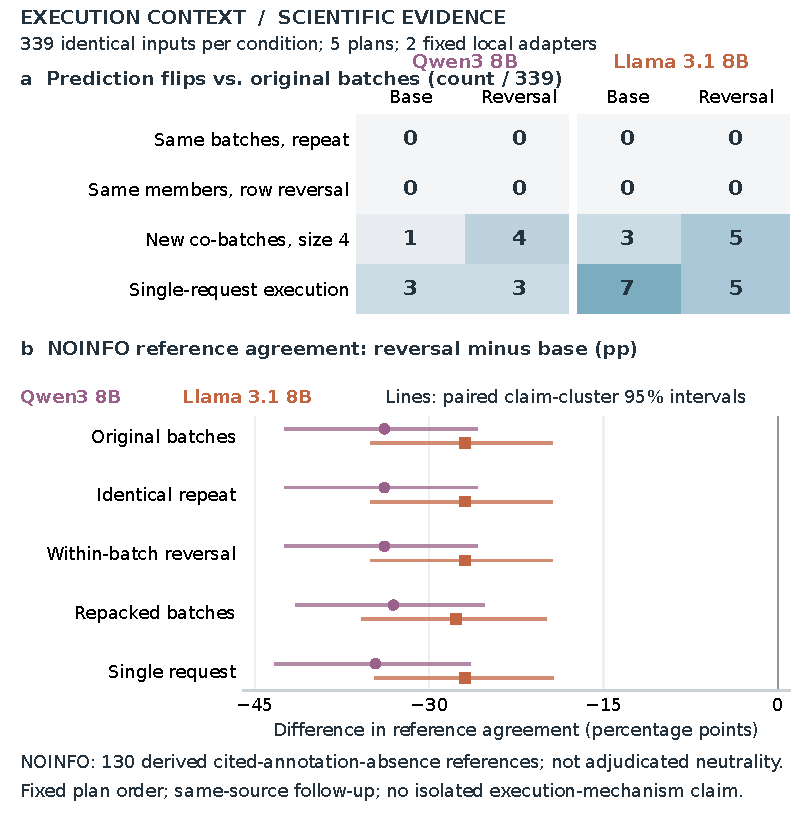
\includegraphics[width=.99\linewidth]{figures/fig_batch_context.pdf}
\caption{Execution-context follow-up on all 339 SciFact cited pairs. (a) Same-condition semantic flips relative to original contiguous batches; columns distinguish base and joint option reversal. (b) Reversal-minus-base reference agreement on all 130 derived \textsc{NoInfo} pairs, with 10,000-draw paired claim-cluster percentile intervals. Execution perturbations move few predictions while the class-specific interface effect persists. \textsc{NoInfo} is cited annotation absence, not adjudicated neutrality. Fixed execution-plan order is not counterbalanced.}
\label{fig:batch-context}
\end{figure}

This control supports robustness of the class-level interface pattern to the tested execution contexts, not bitwise determinism or a unique numerical mechanism. Repacking and singleton execution also change padding and kernel shapes; the fixed plan order does not isolate time-dependent effects. Same-process repeats do not establish cross-process, cross-GPU or cross-version reproducibility. These new outputs remain separate from historical results in \texttt{research/batch\_context\_v1/}.

\paragraph{Reference audit prepared, not completed.} A source-verified blinded work package includes all 130 derived \textsc{NoInfo} pairs plus 15 annotated support and 15 contradiction calibration pairs. Two independently randomized packets omit reference labels, strata and model outputs; independent annotation forms are blank. The workflow retains four-way agreement (including UNCERTAIN), separate derived/calibration statistics, locked form hashes and third-reviewer adjudication. Source-containing packets remain restricted and precisely ignored by version control. No human-validity result is claimed until independent reviewers complete this work.
